\documentclass[conference]{IEEEtran}
\IEEEoverridecommandlockouts
% The preceding line is only needed to identify funding in the first footnote. If that is unneeded, please comment it out.
\usepackage{cite}
\usepackage{amsmath,amssymb,amsfonts}
\usepackage{algorithmic}
\usepackage{graphicx}
\usepackage{textcomp}
\def\BibTeX{{\rm B\kern-.05em{\sc i\kern-.025em b}\kern-.08em
    T\kern-.1667em\lower.7ex\hbox{E}\kern-.125emX}}
\begin{document}

\title{Automatic Code Optimizations on GPU Architectures}

\author{
	\IEEEauthorblockN{Johann Wagner}
	\IEEEauthorblockA{
		\textit{Otto-von-Guericke University} \\
		Magdeburg, Germany\\
		johann.wagner@st.ovgu.de
	}
}


\maketitle

\begin{abstract}
	GPU programming is a hot topic. More and more tasks requiring a lot of computing power are performed on graphics cards, such as bitcoin mining. Optimizations that make these applications even more efficient to take full advantage of the power of the graphics cards are all the more important.
	
	After a short introduction to parallel programming and NVIDIA CUDA, this paper compares different approaches to shortening the time a thread waits for memory. There are several optimizations, such as thread block merging, thread merging, data prefetching and the elimination of partition camping. These four optimizations are compared in four different categories.
	
	At the moment there are many implementations that offer improved compilers for CUDA, but few comparisons between different optimizations and their modes of action and lines of action. This paper aims to give an overview of the most important optimizations and to compare them in interesting and simple categories.
\end{abstract}

\begin{IEEEkeywords}
GPU Compiler Optimizations
\end{IEEEkeywords}


% Cite before Point.

\section{Introduction}

	% What is the problem?
		% Complex Calculations, that does not share much data and can be multithreaded.
		% Processing with GPU for Acceleration
		% Optimization is quite basic for GPGPU Compiler at the moment.

	General Purpose Computation on Graphics Processing Unit (GPGPU) is a frequently used term in data processing. Due to this, complex calculations can be accelerated by using GPU instead of CPU.
	
	Todays compilers for CPU architectures are optimized a lot. There are many generally known optimizations like loop unrolling and constant precalcuation. The aim is to avoid problems of CPUs, such as costly instructions like jump- and division-operations \cite{gccoptimizations}.
	
	Loop unrolling tries to get rid of jump-operations, that in the best case accelerates the assembler code by unrolling a loop to procedural code without jump-operations \cite{gccoptimizations}. Constant precalcuation tries to evaluate a formula as best as possible without known variables \cite{gccoptimizations}.
	
	In general, these optimizations try to avoid cost-intensive operations. These are either avoided or calculated at compile time, so that the actual program runs faster. 
	
	Compilers, which are used to create GPGPU applications, have to help the developer more than conventional CPU applications. The main problem with GPGPU applications is memory access. NVIDIA introduces CUDA, a programming model that allows developers to run code on graphics cards, but CUDA introduces six different types of memory, all of which have to be managed by the programmer, which is much more than traditional programming. In addition, this memory access is slow in case of incorrect handling \cite{nvc} \cite{cudap}.
	
	Obviously, other problems have to be solved than with CPU applications. In GPGPU applications, memory access to global memory is the main problem and a problem that can be solved in different ways.
	Therefore, we would like to discuss here what optimizations already exist for the GPU \cite{nvc} \cite{cudap}.
	
	% Why is it interesting and important?
		% Speed up GPGPU code
		% Programming GPU is more complex as CPU Programming
			% Multithreading 
			% 6 Different Memory Types
			% Hard to write performant code
		
	
			
	% Why is it hard? (E.g., why do naive approaches fail?)
		% ?
	% Why hasn't it been solved before? (Or, what's wrong with previous proposed solutions? How does mine differ?)
		% No qualitative comparisions between different GPU Optimizations 
	% What are the key components of my approach and results? Also include any specific limitations.
		% Optimization for Memory Access Times
		% Only Compiler Optimization

	

\section{Background}

	This section is intended to provide an introduction to the various terms used in this paper. The terms Thread and Thread Blocks and General Purpose Computation on GPUs are explained. In addition, NVIDIA CUDA and the different types of memory introduced by CUDA will be presented to help improve understanding of the topic.

	\subsection{Threads and Thread Blocks}
	
	\subsubsection{Threads}
	Threads are subroutines, so a small set of instructions, which can be managed and executed independently from other threads. Threads typically have an independent stack for local variables and share heap with all other threads. Due to access from multiple independent threads, heap access must be managed  \cite{threadDefinition}.
	
	
	\subsubsection{Thread Blocks}
	Thread Blocks is a construct, which was introduced by CUDA to organize threads in groups. Threads, that are grouped in a thread block, can access a part of the storage simultaneously \cite{cudap}.
	
	\subsubsection{Hardware Implementation}
	NVIDIA GTX 1080 has 20 multiprocessors with 128 threads each. This means that the threads of 20 thread blocks can be executed simultaneously. If there are more than 20 thread blocks, they are executed one after the other.
	That means, that 2560 threads can be executed in parallel \cite{1080gtxdepth}.
	
	
	
	\subsection{General Purpose Computation on GPUs}
		
		% Real Intro
		
		% TODO
		
		% Intro with Point - I tried
		Big Computations need a lot of calculation time. Those computations can be mostly splitted into multiple smaller workloads, which can be calculated independently \cite{GPGPUCompiler}. While CPUs are designed to calculate bigger workloads with less threads, GPUs are designed to calculate smaller workloads on hundreds of threads. In its original form, each pixel could be calculated individually on a GPU, which implies heavy multi threading \cite{myth}.
		
		% Punchline 
		
		% Discussion of Advantages, Disadvantages of GPGPU
		
		There are some advantages and disadvantages of GPGPU usage:
		
		\subsubsection{Threading} A problem usually contains multiple smaller workloads, that can be calculated independently on GPUs. This calculations can be processed parallel to save time. Modern GPUs have more than 2500 cores with up to 1.7 GHz, which can execute code parallel. Other papers determine speedups up to 20 times \cite{1080gtx} \cite{speedup}.
		
		
		\subsubsection{Data Transfer Time}  Transferring data from memory into GPU memory is usually a bottleneck. Calculations, which use data from secondary storage or produce a lot of data, have to transfer data to the host system, that moves the data to CPU memory or on secondary storage.
		
		The problem here is the PCIe connection, which is currently specified with a maximum data rate of 32 GB per second. Thus it takes at least 250ms to fill the entire memory of a current graphics card, which is relatively slow in the context of fast calculations \cite{1080gtx} \cite{transferspeedup}.
		
		
		\subsubsection{Complexity} Complexity is a big difficulty. The greater the degree of complexity, the more difficult and slower the development process.  Especially when programming GPUs, the complexity is high and the quality of the programming is decisive for the speed of the application. However, code is often not optimized when the consumer can cope with the waiting time, because the development of accelerated solutions would cost a lot of money \cite{cudalite}.
		
		% Explanation, why GPGPU is interessting
			% Multithreading
		% Advantages, Disadvantages of GPGPU
			% Transfer
			% Complexity
			% Speed
			% Threads
			
		% Conclusion - One Punch Line
			
	\subsection{NVIDIA CUDA}
		
		NVIDIA CUDA is a parallel computing platform and model, which was developed by NVIDIA to speed up applications by usage of NVIDIA GPUs. For example CUDA can be plugged as library into C programs to make use of a CUDA-capable GPU \cite{cudacpp}.
		
		NVIDIA CUDA, further referred as CUDA, makes it easy to access GPU for general purpose programming by providing functions for different programming languages like C, C++ and Python. It provides simple functions and/or annotations to enable GPU usage. 
	
		\begin{figure}[htbp]
			\centerline{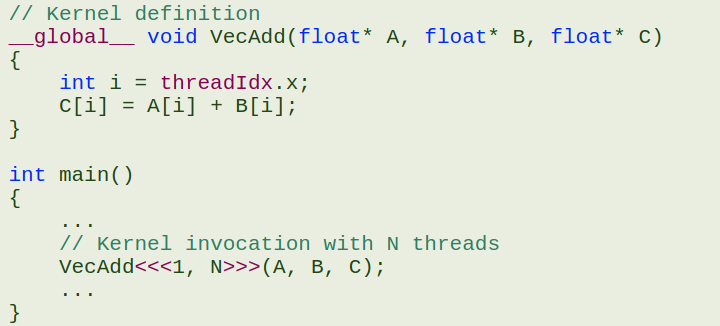
\includegraphics[width=0.4\textwidth]{CudaCode.png}}
			\caption{Code with CUDA Support to add two vectors, accelerated with GPU - Taken from NVIDIA Programming Guide}
			\label{fig}
		\end{figure}

	
		% Explain Figure 1 with Figure 2
		
		In Figure 1, we show a simple vector addition, that is accelerated by using GPU with CUDA. You have to define a kernel function, which is a simple c function, which is called $N$ times by $N$ different CUDA threads. This kernel function is executed on GPU. \texttt{threadIdx.x} contains, in this simple example, just the number (\texttt{ 0 $\leq$ threadIdx.x $<$ N}) of the thread, which called the function. In Figure 2, we show the mathematical equation, which is done by the code in Figure 1. We can calculate every $c_i$ independently in sepeate threads, which makes it possible to speed up the process. This example is trivial, however matrix operations, that are more complex, can be speed up with the same approach \cite{cudap}.
		\begin{figure}[htbp] 
			\begin{align*}
				\begin{pmatrix}
				c_{1} \\
				c_{2} \\
				\vdots \\
				c_{m}
				\end{pmatrix} 
				= 
				\begin{pmatrix}
				a_{1} \\
				a_{2} \\
				\vdots \\
				a_{m}
				\end{pmatrix}
				+ 
				\begin{pmatrix}
				b_{1} \\
				b_{2} \\
				\vdots \\
				b_{m}
				\end{pmatrix}			
			\end{align*}
			\caption{Mathematical Equation for Vector Addition}
		\end{figure}
		
		% General Explanation
			% CUDA is a parallel computing platform and programming model developed by NVIDIA for general computing on graphical processing units (GPUs). With CUDA, developers are able to dramatically speed up computing applications by harnessing the power of GPUs.
		% Advantages of CUDA 
	
	\subsection{Memory Seperation in CUDA}
	
	% http://docs.nvidia.com/cuda/cuda-c-best-practices-guide/index.html#device-memory-spaces__salient-features-device-memory
	
		NVIDIA CUDA introduces six different types of memory, which are up to four more types than in other programming languages. Different types of memory has different attributes.

		\subsubsection{Register}
			Register Memory is quite similar to CPU Register Memory and is used as storage for local variables, etc. It is limited to 16kb and everything, which exceeds this limit, will be pushed on Local Memory \cite{accsql}.
		\subsubsection{Local Memory}
			Local Memory is an abstraction of CUDA, which makes it possible to store information in Global Memory, which is only available from current thread \cite{accsql}.
		\subsubsection{Shared Memory}
			Shared Memory is much faster than the Global Memory. It is visible to all threads, which are in the same thread block. It is intented to share data across multiple threads, that are in the same thread block \cite{cudalite} \cite{cudap}.
		\subsubsection{Global Memory}
			Global Memory is the slowest memory. It is visible to all threads, can be read and written from all threads and can be as General Purpose memory. It is very similar to CPU memory, which makes it easy to use to share data across multiple thread blocks \cite{cudalite}.
		\subsubsection{Constant Memory}
			Constant Memory is quite similar to the Global Memory, but can only be read. It can help to reduce overhead by caching information \cite{cudalite} \cite{accsql}.
		\subsubsection{Texture Memory}
			Texture Memory is quite similar to the Global Memory, but can only be read. It provides some caching methods, which can be used to accelerate certain applications, but this is not used in the further explanations \cite{cudap}.
		
		
		% Explanation about the six different memory types.
		% Categorization with Size, Availability, Speed, Access Time 
		
		% Register
		% Local Memory
		% Shared Memory
		% Global Memory
		% Constant Memory
		% Texture Memory
		


\section{Body}

	Waiting for Memory is one of the most time-consuming states in executing a program. Compared to CPU programming time can be saved in GPU programming by utilizing different memory types, which were introduced in the prior section. Fundamentally data, that is created and used by GPU threads, could be read and written in the global memory. This native approach would be slow, because only one thread could use the data at a time.
	
	It would be better if data that is only used by the thread would also be stored in the memory that can only be used by the thread to reduce memory accesses to global memory and to shorten the wait time for other memory requests for global memory.
	Unfortunately it is not possible to determine the usage of different variables at compile time, because we are not able to test a complex program deterministically, and as a consequence it is not possible to optimize the memory access time this way.

	The primary objective is to keep the time for memory access as short as possible. There are various optimizations for this, such as thread block and thread merging, data prefetching and the elimination of partition camping.
	
	% Punchline	

	% Introduction
	% Why do we want to optimize Memory Access
	% Why do we want to do it automagically
	
	\subsection{Thread-Block Merging}
	
	% Say it, before you say it
	
	Thread merging is a technique where different thread blocks are merged into one thread block to reduce memory access times.
	
	% General Explanation 
	
	Thread Blocks have a shared memory segment, where they can save data for execution. If multiple thread blocks use the same data from the global memory to execute its threads, we can merge them into one thread block to reduce the memory access for global memory \cite{GPGPUCompiler}.
	
	% Graphic for Explanation
	
	In Figure 3, we show an example for merging two thread blocks. Both thread blocks contain a data segment, which is equivalent from global memory. After the merge the data segment is only fetched one time and the number of threads in the thread block adds up.
	
	\begin{figure}[htbp]
		\centerline{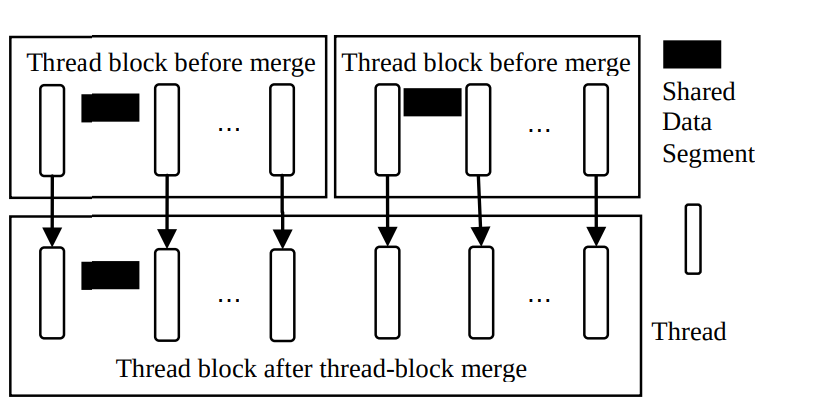
\includegraphics[width=0.4\textwidth]{ThreadBlockMerge.png}}
		\caption{Improved Memory Reuse by Thread Block Merging - Taken from A GPGPU Compiler for Memory Optimization and Parallelism Management}
		\label{fig3}
	\end{figure}
	
	\subsection{Thread Merging}
	
	% Say it, before you say it
	
	Thread merging is a technique where different threads are merged into one thread to reduce memory access times. In exchange, there are less concurrent threads, which reduces the absolute computation time.
	
	% General Explanation 
		

	The goal of thread merging is to reuse data. In the best case, each block of data has to be fetched only once. In addition to thread block merging, which only allows for the reuse of Shared Data Segments, thread merging allows the reuse of shared registers too \cite{GPGPUCompiler}. 
	
	% Graphic for Explanation
	
	In Figure 4, we show an example for merging two thread blocks into one thread block by merging threads. Again, both blocks contain a shared data segment, which is equivalent. Additionally a shared register per thread is equivalent. By merging two threads into one, the shared data segment and the shared register just have to be fetched once.
	
	\begin{figure}[htbp]
		\centerline{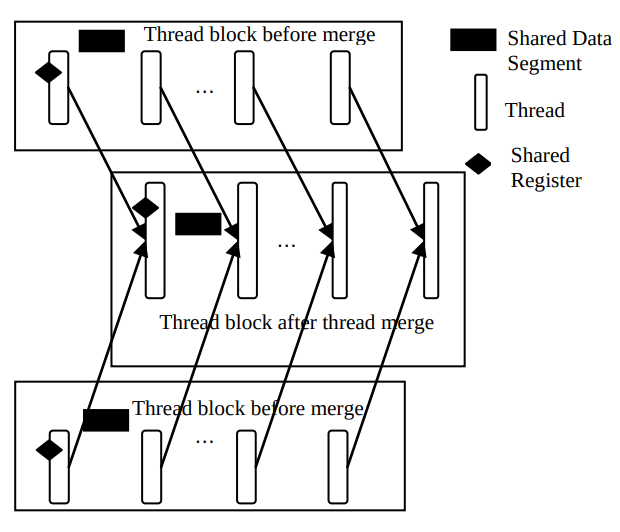
\includegraphics[width=0.4\textwidth]{ThreadMerge.png}}
		\caption{Improved Memory Reuse by Thread Merging - Taken from  A GPGPU Compiler for Memory Optimization and Parallelism Management}
		\label{fig2}
	\end{figure}
	


	\subsection{Data Prefetching}
		
		% Say it, before you say it
		
		Data prefetching is a technique to optimize loops by prefetching the data, before they are actually needed.
		
		% General Explanation
		
		Data prefetching optimizes the iteration over data structures by prefetching the data, that is needed in the following iteration step. In the current iteration step $i$ the data from iteration step $i+1$ gets fetched. This step allows you to overlap memory access time and computing time \cite{GPGPUCompiler}. In exchange the actual iteration step become slower by adding some extra instructions for prefetching.
		
		In Figure 5, we show example code with data prefetching. The code is part of the code for matrix multiplication. To understand the concept the $tmp$ variable is important. In the beginning $tmp$ holds the first part of data. In the following iteration steps it requests the part of data, that is used in the following step. That is an asynchronous event, that run next to the calculations of the current iteration step. 
		
		\begin{figure}[htbp]
			\centerline{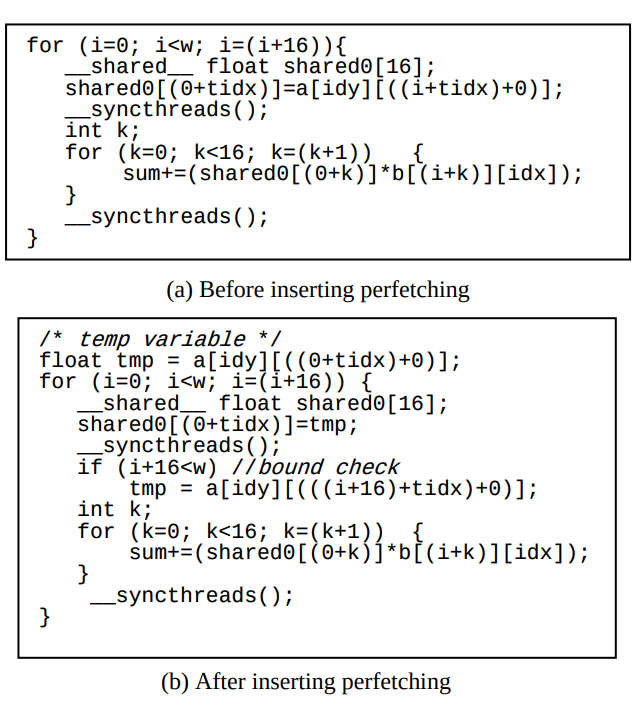
\includegraphics[width=0.4\textwidth]{DataPrefetchingCodeExample.png}}
			\caption{Example Code for Data Prefetching - Taken from  A GPGPU Compiler for Memory Optimization and Parallelism Management}
			\label{fig2}
		\end{figure}
	
		In Figure 6, we show a timeline, that shows the overlapping execution times from fetching data and executing code after the optimization. There is no time saving in the first iteration, because it is not possible to execute code without loaded data. After the first iteration, data can be loaded and code can be executed at the same time.
		
		\begin{figure}[htbp]
			\centerline{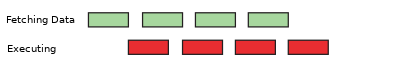
\includegraphics[width=0.4\textwidth]{DataPrefetching.png}}
			\caption{Example Timeline for Example Code in Figure 5 - Taken and Modified from NVIDIA CUDA Programming Guide}
			\label{fig2}
		\end{figure}
		
	\subsection{Partition Camping}
		
		% Say it, before you say it.
		
		Partition Camping is a problem, which is related to the memory architecture of NVIDIA CUDA. It describes the problem, that data, that is used in different threads, uses the same partition in global memory, which implies long memory access times. 
		
		% General Explanation
		
		The global memory of graphics cards is divided into partitions. Partitions can only be read or written by one thread at a time. If several threads want to access a partition at the same time, a queue is created and the threads cannot calculate any further. If all parts of the data set are located on a few partitions, then many threads need to access one partition, so memory access is slower. This is called partition camping \cite{pc} \cite{GPGPUCompiler}.
		
		If the data is evenly distributed across all available partitions, a single partition has fewer threads to access, which speeds up memory access. However, please note that data can only be efficiently redistributed if there is enough space and a good structure of the data.  In addition, it can happen that redistribution makes the code faster in one place, but decelerates other places where the data is used in a different way \cite{pc} \cite{GPGPUCompiler}.
		
		% Graphics
			% Not that easy to understand
		
		In Figure 7, we show $\text{SM-1}, \text{SM-2}, \dots, \text{SM-30}$, which are different accessors. 
		
		In the table titled "Without Partition Camping" we show that the data for the different accessors are distributed evenly over all partitions. 
		
		In the table titled with "With Partition Camping" we show that the data is all in one partition and that all accessors would have to access one partition, resulting in long waiting times.
		
		In conclusion, it can be said that in this example it is very easy to see that the individual partitions are used by considerably fewer accessors, which reduces the waiting time for memory.
			
		\begin{figure}[htbp]
			\centerline{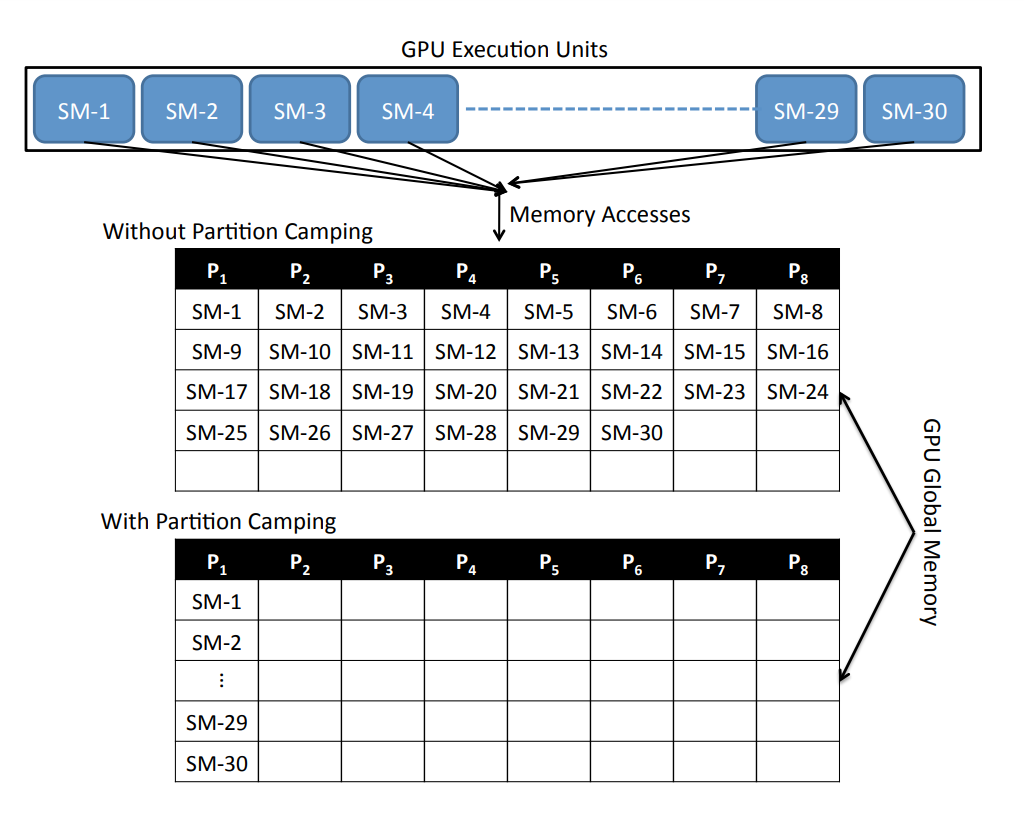
\includegraphics[width=0.4\textwidth]{PartitionCamping.png}}
			\caption{Partition Camping Example - Taken from Bounding the Effect of Partition Camping in GPU Kernels}
			\label{fig2}
		\end{figure}

\section{Evaluation}

	% Go through Categories and categorize every Optimization for every Category and explain why.
	% Categories
		% Use Cases (special or general)
		% Efficiency
		% Difficulty
		% Code Examples (?)
		% Error Case
	
	In this section we compare the different optimizations for GPGPU, which we have explained before. In doing so, we will look at various points such as use cases, efficiency, difficulty and error cases. Note that all optimizations occur at compile time and do not mean any additional work for the developer of the application.
	
	\begin{figure}[htbp]
		\centerline{
			\begin{tabular}{ c | c | c | c | c }
				Optimization & UC & E & D & EC \\ \hline
				Thread Block Merge & - & + & - & \\
				Thread Merge & - & + & - & \\
				Data Prefetching & + & - & + & \\
				Eliminiation of Partition Camping & + & o & + & \\
			\end{tabular}
		}
		\caption{Comparison of different optimizations - Use Cases (UC), Efficiency (E), Difficulty (D), Error Cases (EC)}
		\label{figtable}
	\end{figure}
	
	
	\subsection{Use Cases}
		Cases for data prefetching and partition camping occur quite frequently. Nearly every loop that accesses data in global memory can be optimized with the help of data prefetching.  The costs of the additional registers required for the temporary variable are relatively low.
		
		The effect of partition camping always occurs when processing relatively large amounts of data and is therefore also optimized.
		
		However, the use cases for thread merging and thread block merging are less frequent, since the circumstances and prerequisites are considerably more complex. Although cases in which these optimizations work can be constructed in this way, the application of this optimization is probably less in comparison to data prefetching.
		
	\subsection{Efficiency}
		The efficiency of the various optimizations can be measured by the increase in speed and number of memory accesses.
		
		Thread merging and thread block merging reduce memory access by the number of $n$ threads merged. This arithmetically increases the speed by a factor of $n$. According to REFERENCE, an acceleration of 10 times is possible in some cases.
		
		The speed increase is not directly calculable with the elimination of partition camping and data prefetching, since it depends on many different factors.
		
		The speed increase for the two other optimizations is much lower in detail, since only increases of the speed are possible in the same example by 2 to 4 times. These two optimizations do not reduce memory accesses.
		
		
	\subsection{Difficulty}
		
		Difficulty describes the effort of implementation for the application developer and the developer of the compiler. In this case, where the compiler automatically optimizes the application, there is no difficulty for the developer of the application, who does not have to work on the optimization.

		The difficulty of data prefetching is, according to REFERENCE, easy to classify. The sample code in Figure 5 shows that the optimization is trivial to implement, apart from the bounding checks.
		
		Implementing the elimination of partition camping is a bit more difficult to evaluate. There are several approaches to better disseminate data that produce different results. However, an initial implementation is relatively simple. 
		Suppose there are $n$ different partitions. Then the data of each partition can be split $m$ times, so that it can be distributed to $n$ partitions. Each partition contains an average of $m/n$ data blocks.
		
		
		Unfortunately, there is little information about the difficulty of implementing Thread Block Merging and Thread Merging. The detection is also not explained further, so that no conclusions can be drawn.
		
	
	\subsection{Error Cases}
	
	
\section{Related Work}

	Yi Yang et. al. wrote a paper on "A GPGPU Compiler for Memory Optimization Parallelism Management" which explains how to implement the optimizations presented in this paper. Further optimizations are also presented and these optimizations are tested using examples such as matrix multiplication with large matrices \cite{GPGPUCompiler}.
	
	Ashwin M. Aji et al. wrote an article on "Bounding the Effect of Partition Camping in GPU Kernels", which explains the effect of Partition Camping in more detail. It also explains the different patterns that can be used to avoid partition camping, which have been omitted in this paper for reasons of simplicity \cite{pc}.  
	
	This paper optimizes access to shared storage areas.  Greg Ruetsch et. al. from NVIDIA have carried out several optimizations using the example of matrix multiplication. An optimization was that the data is stored in such a way that no conflicts occur, which is a further development and/or modification of the partition camping solution \cite{mtransnvidia}.
	
\section{Conclusion}
	

\begin{thebibliography}{00}
\bibitem{nvc} CUDA Zone - https://developer.nvidia.com/cuda-zone
\bibitem{GPGPUCompiler} Yi Yang, Ping Xiang, Jingfei Kong, Huiyang Zhou, "A GPGPU Compiler for Memory Optimization and Parallelism Management", 2010
\bibitem{myth} Victor W Lee, Changkyu Kim, Jatin Chhugani et. al "Debunking the 100X GPU vs. CPU Myth: An Evaluation of Throughput Computing on CPU and GPU", 2010
\bibitem{1080gtx} NVIDIA GeForce GTX 1080, https://www.nvidia.com/en-us/geforce/products/10series/geforce-gtx-1080/
\bibitem{1080gtxdepth} NVIDIA GeForce GTX 1080 White Paper,
https://international.download.nvidia.com/geforce-com/international/pdfs/GeForce\_GTX\_1080\_Whitepaper\_FINAL.pdf
\bibitem{cudacpp} GPU Accelerated Computing with C and C++ - https://developer.nvidia.com/how-to-cuda-c-cpp
\bibitem{cudap} Programming Model - Kernel http://docs.nvidia.com/cuda/cuda-c-programming-guide/index.html\#kernels
\bibitem{cudalite} Sain-Zee Ueng, Melvin Lathara, Sara S. Baghsorkhi, Wen-mei W. Hwu, "CUDA-Lite: Reducing GPU Programming", 2008
Complexity
\bibitem{accsql} Peter Bakkum, Kevin Skadron, "Accelerating SQL Database Operations on a GPU with CUDA", 2010
\bibitem{pc} Ashwin M. Aji, Mayank Daga, Wu-chun Feng, "Bounding the Effect of Partition Camping in GPU Kernels", 2011
\bibitem{mtransnvidia} Greg Ruetsch, Paulius Micikevicius, "Optimizing Matrix Transpose in CUDA", 2009 
\bibitem{gccoptimizations} GCC Optimize Options - https://gcc.gnu.org/onlinedocs/gcc/Optimize-Options.html
\bibitem{threadDefinition}  Lamport, Leslie (September 1979). "How to Make a Multiprocessor Computer That Correctly Executes Multiprocess Programs" (PDF). IEEE Transactions on Computers. C–28 (9): 690–691. doi:10.1109/tc.1979.1675439.



\end{thebibliography}

\end{document}

